% This file was autogenerated from the template: documentation.tex.template (2022-10-10 15:54:03).

\documentclass[10pt,a4paper]{article}
\usepackage[english]{babel}
\usepackage[utf8]{inputenc}
\usepackage{amsmath}
\usepackage{amsfonts}
\usepackage{amssymb}
\usepackage{graphicx}
\usepackage{float}
\usepackage{hyperref}

%link to documentation: 
%https://ackrep-doc.readthedocs.io/en/latest/devdoc/contributing_data.html

\begin{document}
	\part*{Model Documentation of the \\ 'CD player SLICOT Working note 2002-2'} % MUST - Add Model Name 
	
	%%%%%%%%%%%%%%%%%%%%%% NOMENCLATURE %%%%%%%%%%%%%%%%%%%%%%%%%%%
	
	\section{Nomenclature} % MUST
	\subsection{Nomenclature for Model Equations} % MUST
	
	%variables for model equations
	\begin{tabular}{ll}
		$x$ & state vector \\
		$u$ & control input vector \\
		$w$ & noise vector \\
		$z$ & regulated output vector \\
		$y$ & measurement vector \\
		
				
	\end{tabular}
	 

	
	%%%%%%%%%%%%%%%%%%%%%% MDOEL EQUATIONS %%%%%%%%%%%%%%%%%%%%%%%%%%%
	
	\section{Model Equations} % MUST
	
	State Vector and Input Vector:
	\begin{align*}
		x &\in\mathbb{R}^120
		u &\in\mathbb{R}^2
		w &\in\mathbb{R}^2
		z &\in\mathbb{R}^4
		y &\in\mathbb{R}^2
	\end{align*}
	
	\noindent System Equations:			
	\begin{subequations}
	\begin{align}
		\dot{x}(t) &= Ax(t) + B_1w(t) + Bu(t) \\
		z(t) &= C_1x(t) + D_{11}w(t) + D{12}u(t) \\
		y(t) &= Cx(t) + D{21}w(t)
	\end{align}
	\end{subequations}

	%%%%%%%%%%%%%%%%%%%%%% PARAMETERS | OUTPUTS %%%%%%%%%%%%%%%%%%%%%%%%%%%
	\noindent
	Outputs: $z$ % MAY
	
	
	%%%%%%%%%%%%%%%%%%%%%% EXEMPLARY PARAMETER VALUES %%%%%%%%%%%%%%%%%%%%%%%%%%%	
	
	\subsection{Exemplary parameter values}
	\begin{tabular}{cl}
\hline
  Symbol  & Value                                                                                                                                                                                \\
\hline
   $A$    & $\left[\begin{matrix}0.8189 & 0.0863 & 0.09 & 0.0813\\0.2524 & 1.0033 & 0.0313 & 0.2004\\-0.0545 & 0.0102 & 0.7901 & -0.258\\-0.1918 & -0.1034 & 0.1602 & 0.8604\end{matrix}\right]$ \\
   $B$    & $\left[\begin{matrix}0.0045 & 0.0044\\0.1001 & 0.01\\0.0003 & -0.0136\\-0.0051 & 0.0936\end{matrix}\right]$                                                                          \\
 $B_{1}$  & $\left[\begin{matrix}0.0045 & 0.0044\\0.1001 & 0.01\\0.0003 & -0.0136\\-0.0051 & 0.0936\end{matrix}\right]$                                                                          \\
 $C_{1}$  & $\left[\begin{matrix}1.0 & 0 & -1.0 & 0\\0 & 0 & 0 & 0\\0 & 0 & 0 & 0\end{matrix}\right]$                                                                                            \\
   $C$    & $\left[\begin{matrix}1.0 & 0 & 0 & 0\\0 & 0 & 1.0 & 0\end{matrix}\right]$                                                                                                            \\
 $D_{11}$ & $\left[\begin{matrix}0 & 0 & 0\\0 & 0 & 0\\0 & 0 & 0\end{matrix}\right]$                                                                                                             \\
 $D_{12}$ & $\left[\begin{matrix}0 & 0\\1.0 & 0\\0 & 1.0\end{matrix}\right]$                                                                                                                     \\
 $D_{21}$ & $\left[\begin{matrix}0 & 1.0 & 0\\0 & 0 & 1.0\end{matrix}\right]$                                                                                                                    \\
\hline
\end{tabular}

	%%%%%%%%%%%%%%%%%%%%%% DERIVATION & EXPLANATION %%%%%%%%%%%%%%%%%%%%%%%%%%%	
	
	\section{Derivation and Explanation} % SHOULD
This model is part of the \href{http://www.compleib.de/}{"`COMPleib"' - library} and wasautomatically imported into ACKREP.\\The original description was:\\CDP CD player SLICOT Working note 2002-2 Y. Chahlaoui, P. Van Dooren --\textgreater{} Ex. 2.3 W. Draijer, M. Steinbuch, O.H. Bosgra and "Adaptive control of the radial servo system of a compact disc player" Automatica, Vol. 28, No. 3, pp. 455-462, 1992

\section{Simulation}
\begin{figure}[H]
\centering
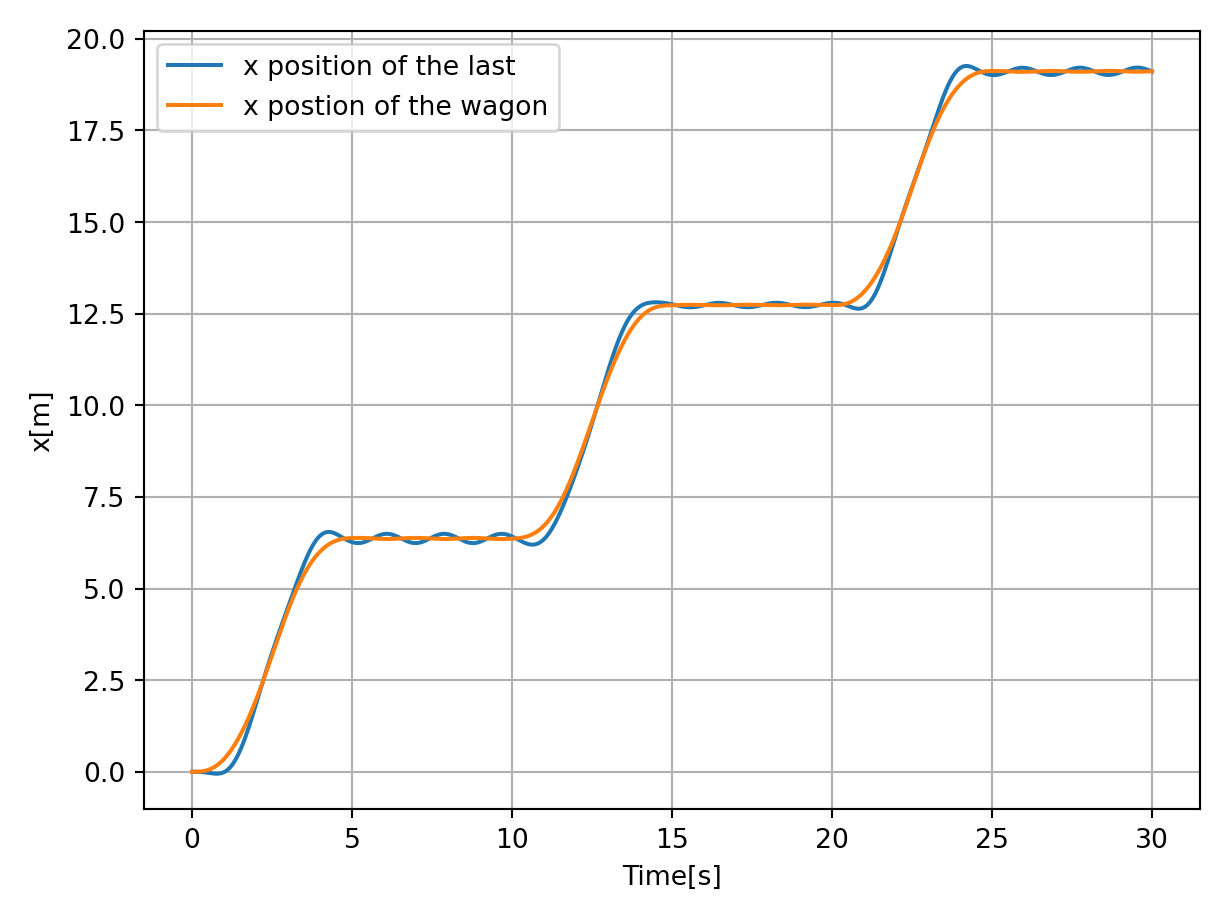
\includegraphics[width=\linewidth]{C:/Users/Julius Fiedler/Documents/Code/ackrep/ackrep_data/../ackrep_data/system_models/compleib_models/CDP/_data/plot.png}
\caption{Simulation of the CD player SLICOT Working note 2002-2.}
\end{figure}
\begin{thebibliography}{10}		
		\bibitem Y. Chahlaoui, P. Van Dooren --> Ex. 2.3 W. Draijer, M. Steinbuch, O.H. Bosgra and "Adaptive control of the radial servo system of a compact disc player" Automatica, Vol. 28, No. 3, pp. 455-462, 1992
	\end{thebibliography}

\end{document}
